\documentclass[12pt]{article}
\textwidth 15.5cm \oddsidemargin 0cm \topmargin -1cm \textheight
24cm \footskip 1.5cm \usepackage{epsfig}
\usepackage{amsmath, graphicx, psfrag, pstcol, float, listings}
\def\n{\noindent}
\def\u{\underline}
\def\hs{\hspace}
\newcommand{\thrfor}{.^{\displaystyle .} .}
\newcommand{\bvec}[1]{{\bf #1}}
\newcommand{\code}[1]{\texttt{#1}}

\begin{document}

\noindent
\rule{15.7cm}{0.5mm}


\begin{center}
{\bf ENGINEERING TRIPOS PART II A}
\end{center}
\vspace{0.5cm} {\bf EIETL \hfill MODULE EXPERIMENT 3F3}
\vspace{0.5cm}
\begin{center}
{\bf RANDOM VARIABLES and RANDOM NUMBER GENERATION\\
Short  Report \\\hfill \\Name: Harry Sarson \\\hfill\\
College: Pembroke \\\hfill
\\
Date: 03/11/2017
}
\end{center}
\rule{15.7cm}{0.5mm}

\pagebreak

\begin{enumerate}
\item {\bf Uniform and normal random variables.}

Histogram of Gaussian random numbers overlaid on exact Gaussian curve (scaled):
 

\begin{figure}[H]
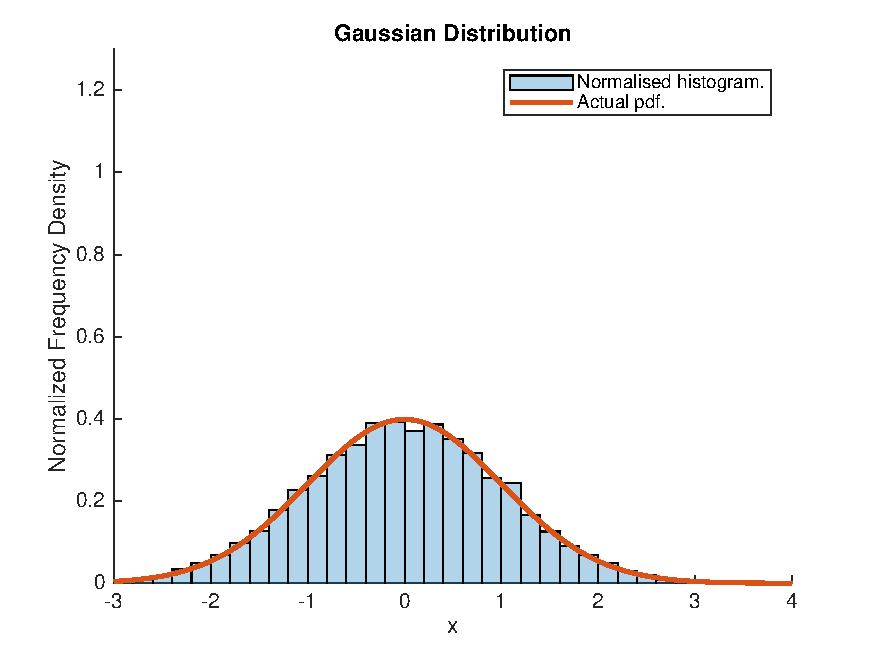
\includegraphics[width=\textwidth]{figures/gaussian-histogram.pdf}
  \caption{Histogrammed samples taken from a Gaussian distribution.}
  \label{fig:gaussian-histogram}
\end{figure}

Histogram of Uniform random numbers overlaid on exact Uniform curve (scaled):


\begin{figure}[H]
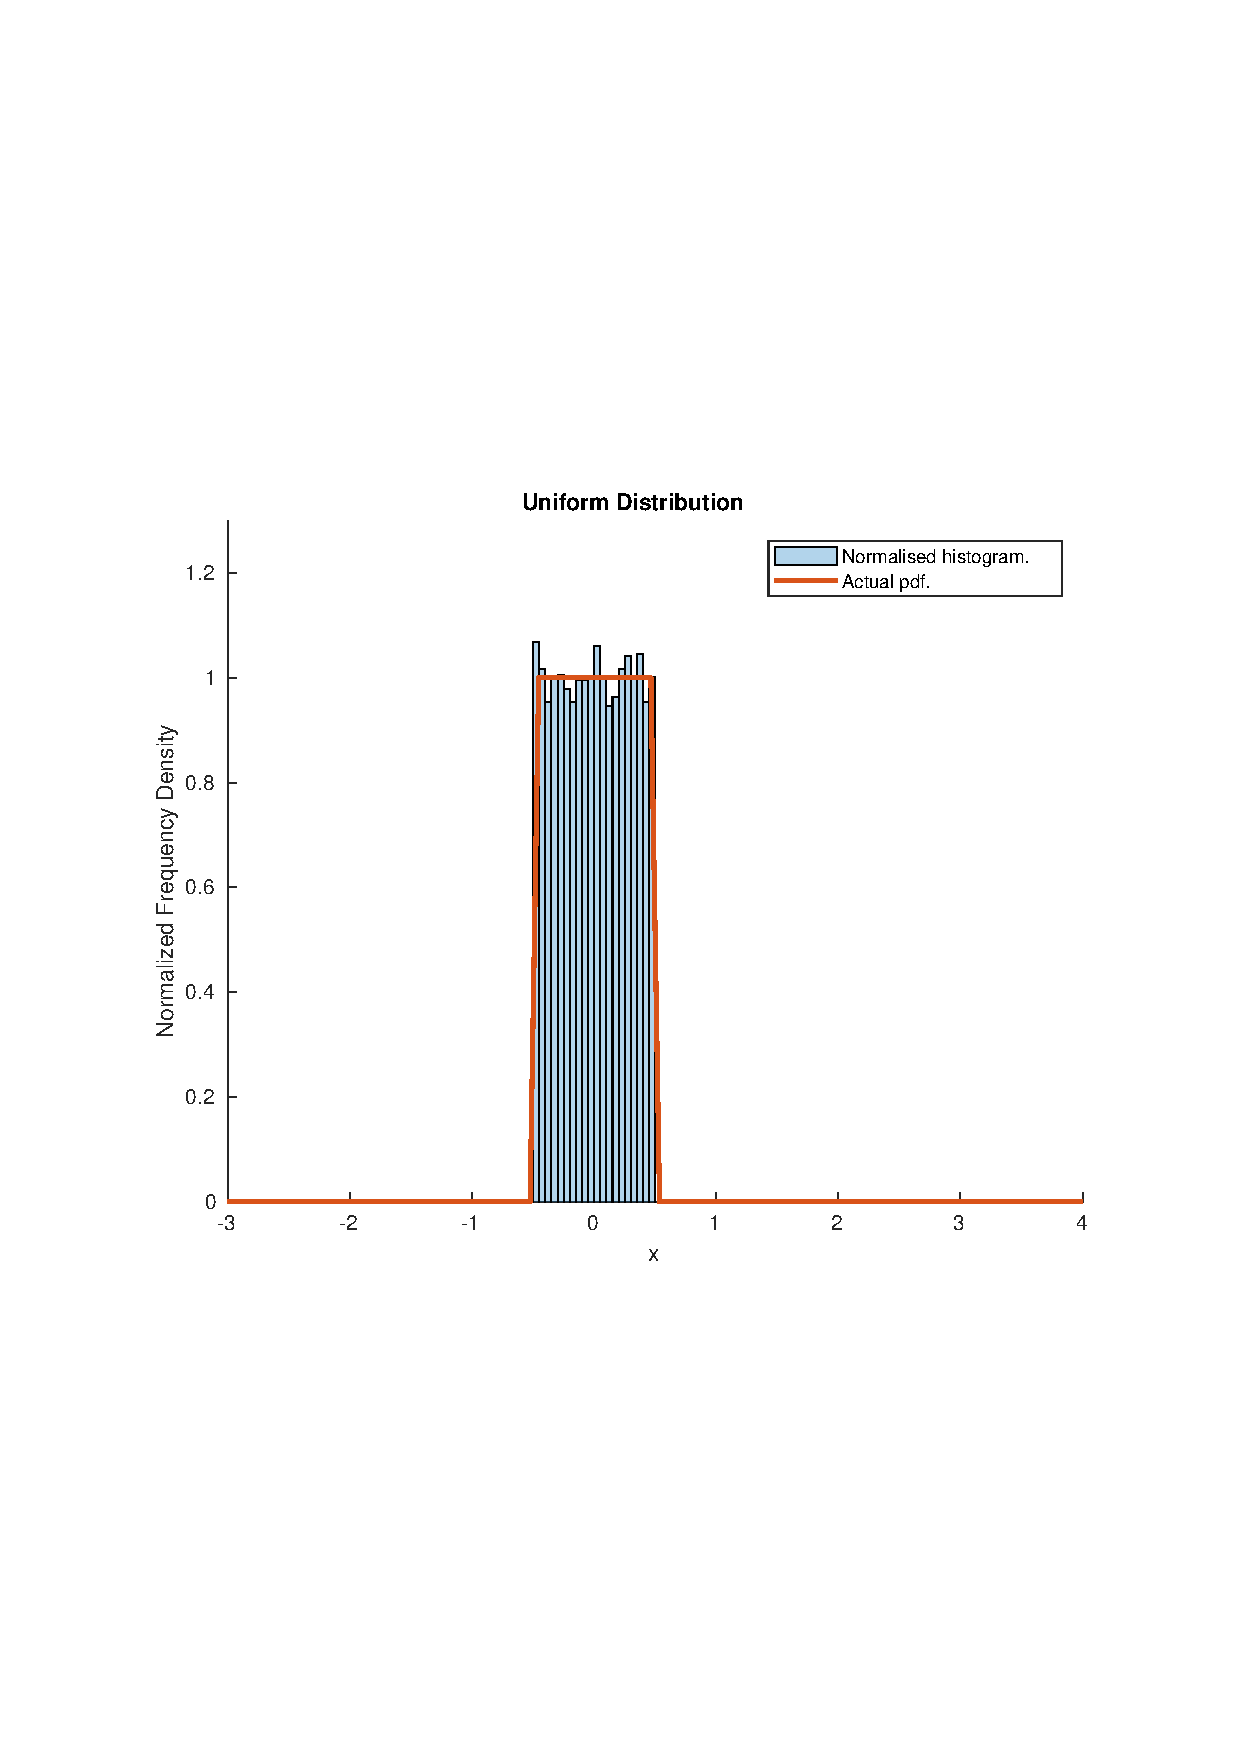
\includegraphics[width=\textwidth]{figures/uniform-histogram.pdf}
  \caption{Histogrammed samples taken from a Uniform distribution.}
\end{figure}
\item 



Kernel density estimate for Gaussian random numbers overlaid on exact Gaussian curve:


\begin{figure}[H]
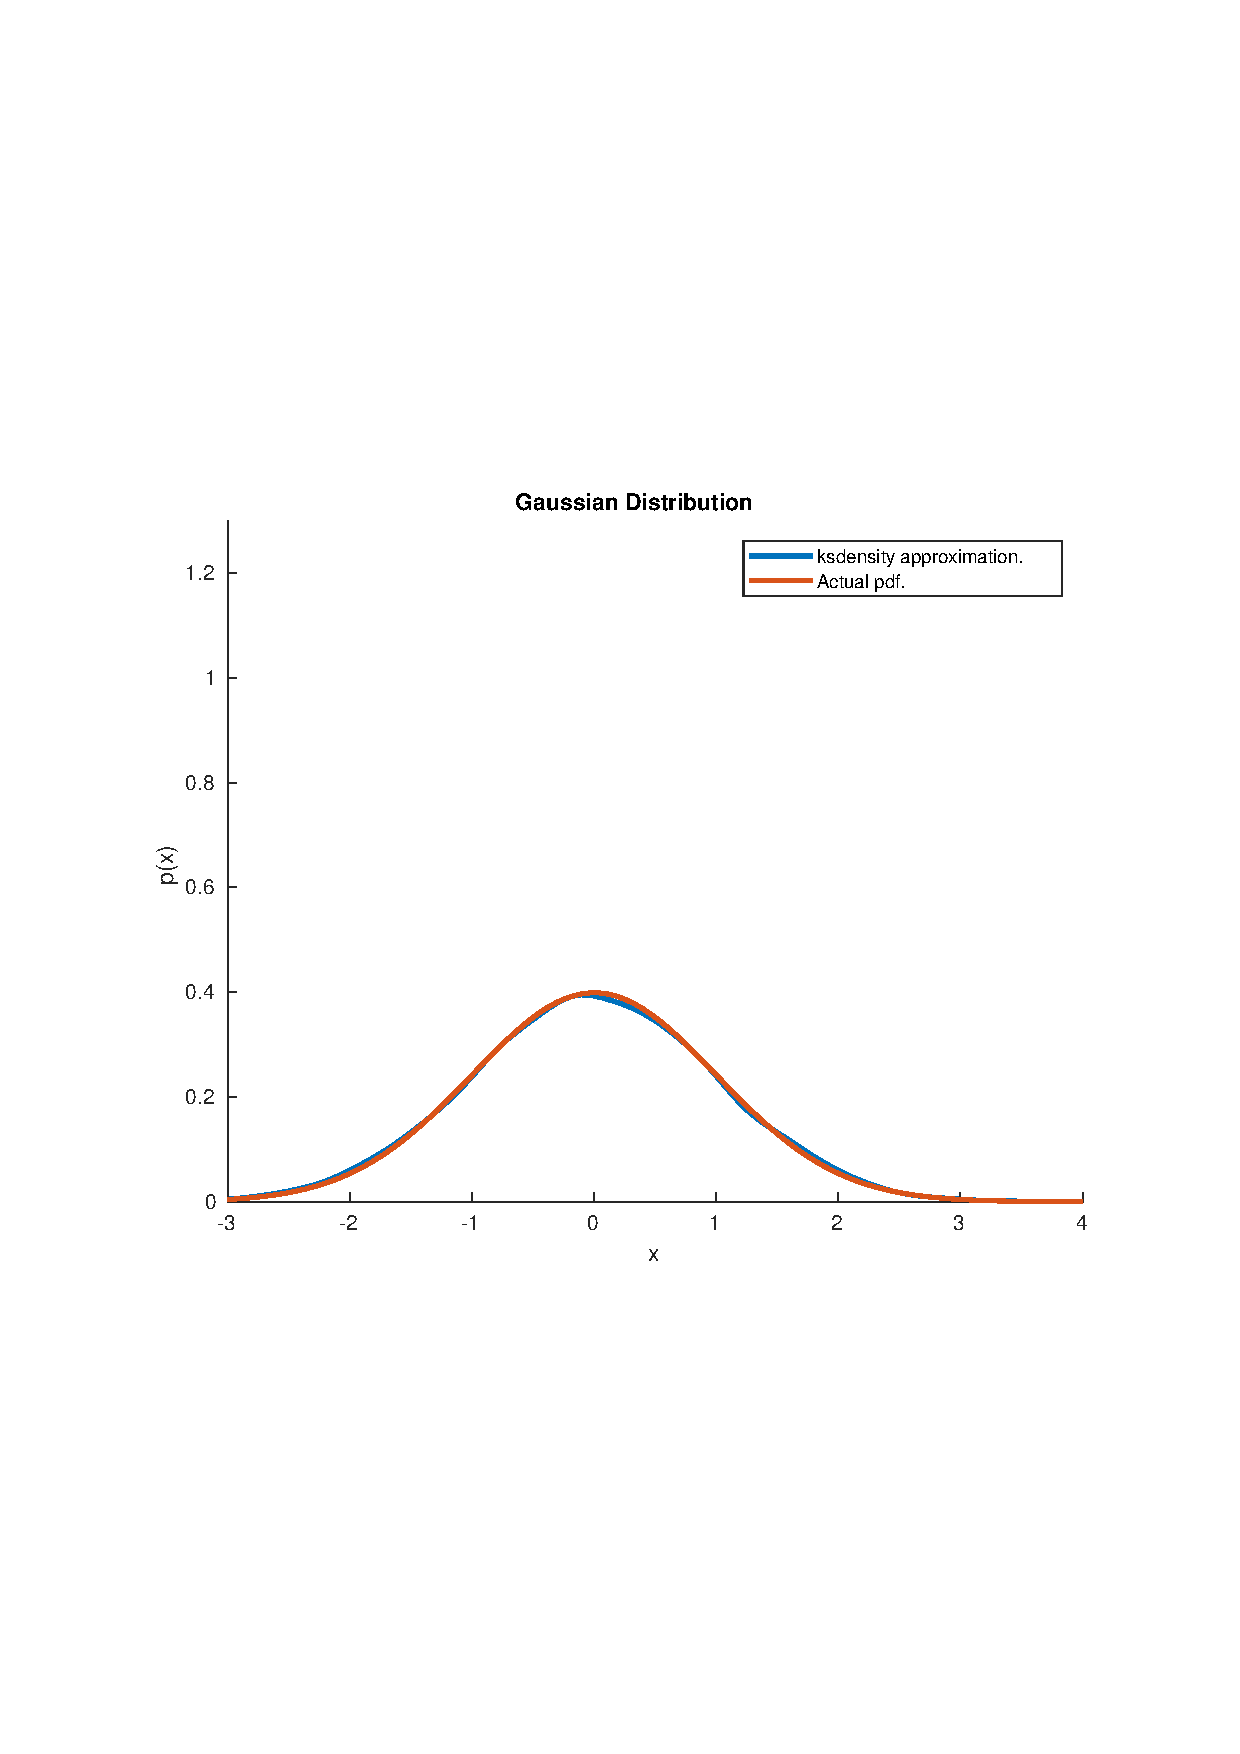
\includegraphics[width=\textwidth]{figures/gaussian-ksdensity.pdf}
  \caption{\code{ksdensity} estimate of Gaussian PDF.}
\end{figure}



Kernel density estimate for Uniform random numbers overlaid on exact Gaussian curve:


\begin{figure}[H]
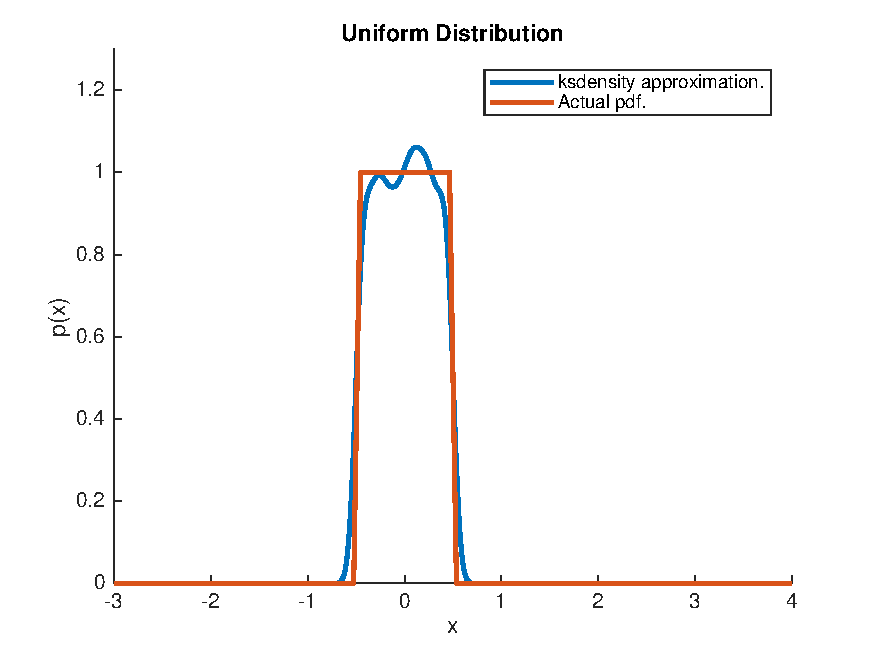
\includegraphics[width=\textwidth]{figures/uniform-ksdensity.pdf}
  \caption{\code{ksdensity} estimate of Gaussian PDF.}
\end{figure}

The \code{ksdensity} method is effective if the PDF is smooth (for example a Gaussian PDF) but is unsuitable for PDFs including discontinuities which it overly smoothes. This is because the \code{ksdensity}'s use of Gaussian kernels causes it to act as a low pass filter and therefore cannot be used with PDFs containing high frequencies (i.e. discontinuities).



Theoretical mean and standard deviation calculation for uniform density as a function of $N$:

For a uniform distribution the histogram count data (the heights of unnormalized bars on a histogram plot) will be multinomially distributed. The probability $p_j$ of a sample  $x^{(i)}$ lying in a bin is equal to the width of the bin divided by the total width of the distribution. Therefore, $p_j = 1/J$ where $J$ is the total number of bins.

For a histogram of samples of a uniform random variable.

\begin{itemize}
\item The mean bar height  $\mu = NJ$
\item The variance in bar height $\sigma^2 = NJ(1-J)$.
\end{itemize}


The ratio $\frac \sigma \mu = \sqrt \frac{(1-J)}{NJ}$ and so as $N \to \infty$, $\frac \sigma \mu \to 0$


Plots of histograms for $N=100$,  $N=1000$ and $N=10000$ with theoretical mean  and $\pm 3$ standard deviation lines:


\begin{figure}[H]
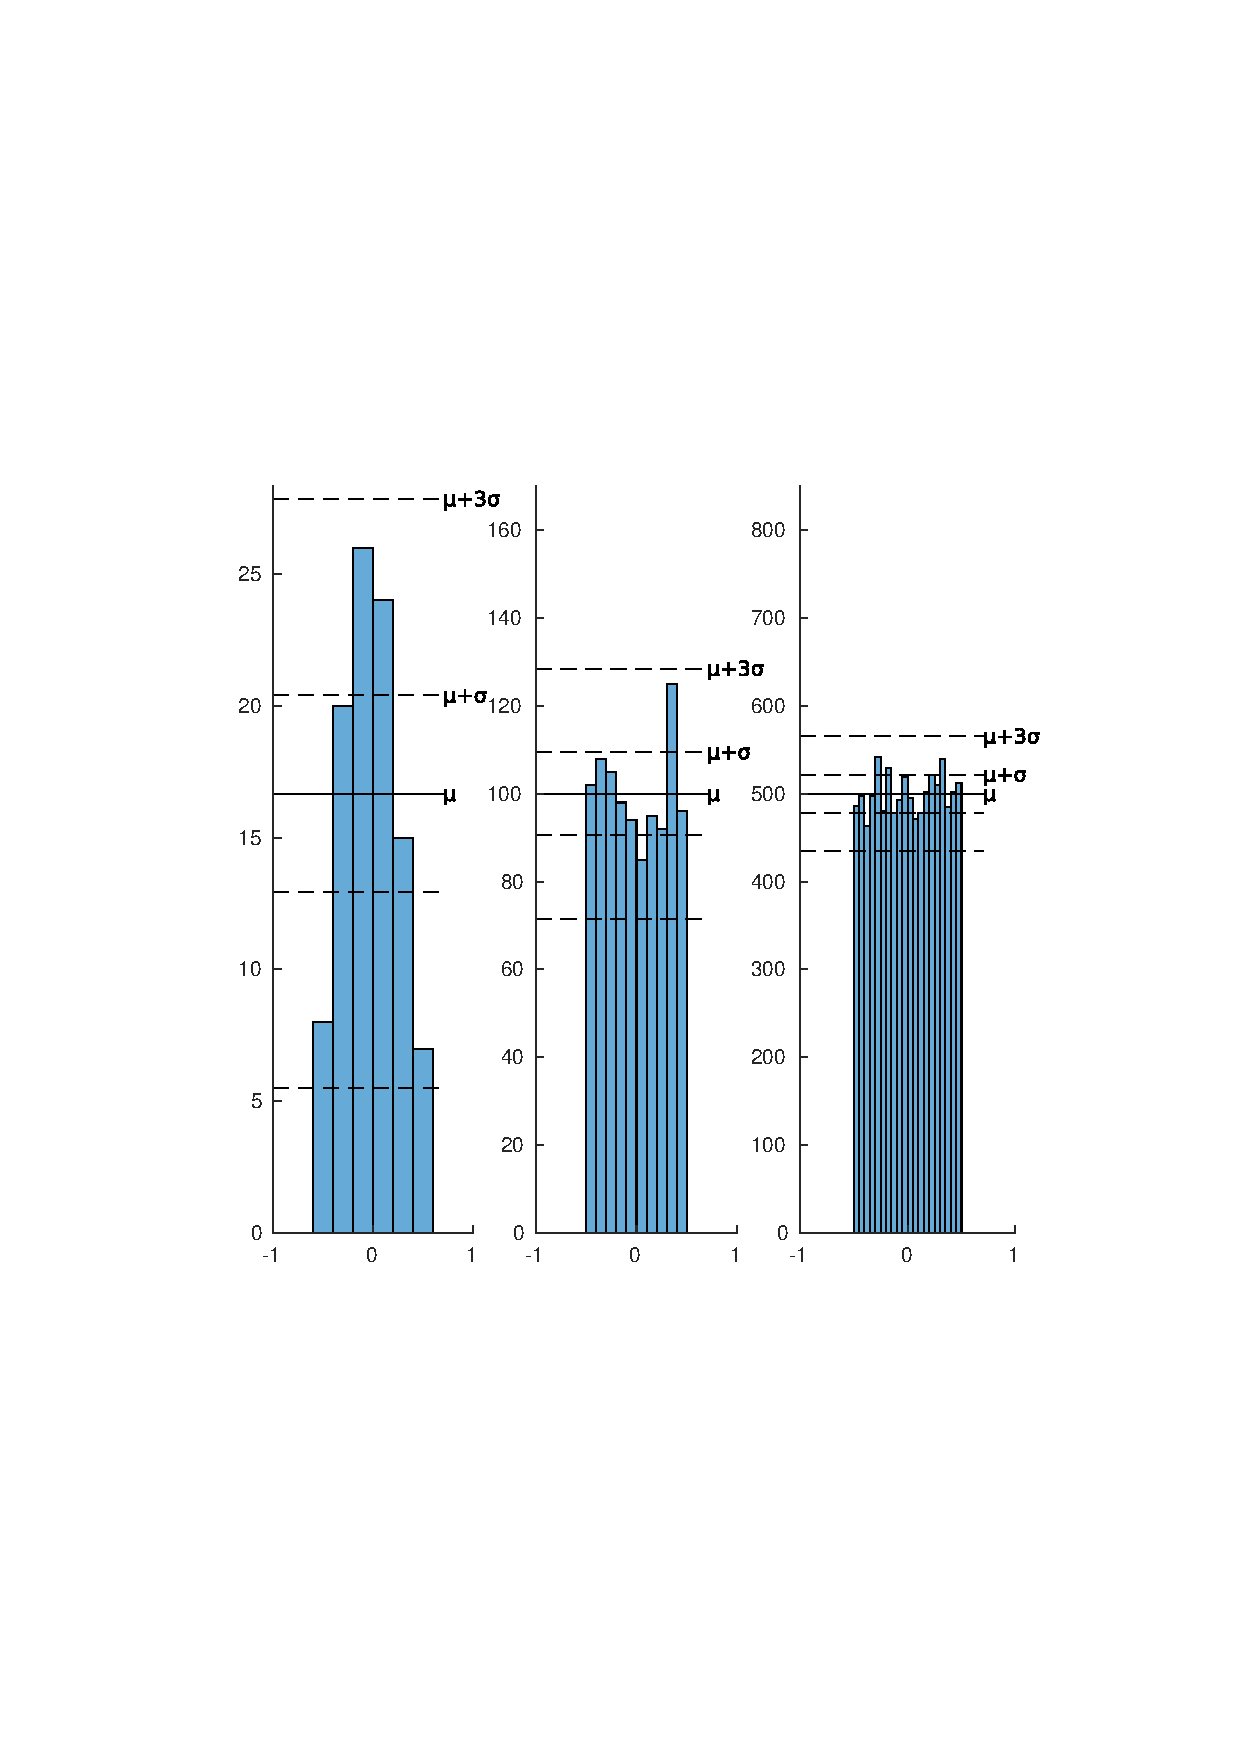
\includegraphics[width=\textwidth]{figures/uniform-bar-distribution.pdf}
  \caption{Histograms of uniformly distributed samples showing mean and standard deviation lines.}
  \label{fig:hist-dist}
\end{figure}


All the histogram bars are within three standard deviations from the mean and the majority of histogram bars are within one standard deviation from the mean. From the three plots in figure \ref{fig:hist-dist} it can be seen that the standard deviation increases with $N$ but the ratio of the standard deviation to the mean decreases.


\item {\bf Functions of random variables}
For normally distributed $X \sim {\cal N}(x|0,1)$ random variables, take $y=f(x)=ax+b$.


\begin{align*}
p_Y(y) &= \left. \frac {p_X(x)} {\frac {dy} {dx}} \right|_{x = f^ {-1} (x)} \\
f(x) &= ax + b \\
f^{-1}(y) &= \frac{y - b} a \\
p_Y(y) &= \frac {p_X \left (\frac {y - b} a \right)} a
\end{align*}

Therefore $Y \sim {\cal N}(y|b, a^2)$ the linear function $f$ of a Gaussian random variable with 0 mean and unit variance creates a general normal density with non-zero mean and non-unity variance.

Transforming a large collection of random samples $x^{(i)}$ to give $y^{(i)}=f(x^{(i)})$, histogramming the resulting $y$ samples gives figure \ref{fig:gaussian-linear-transform} which verifies the result as the random samples strongly follow the analytically calculated PDF.


\begin{figure}[H]
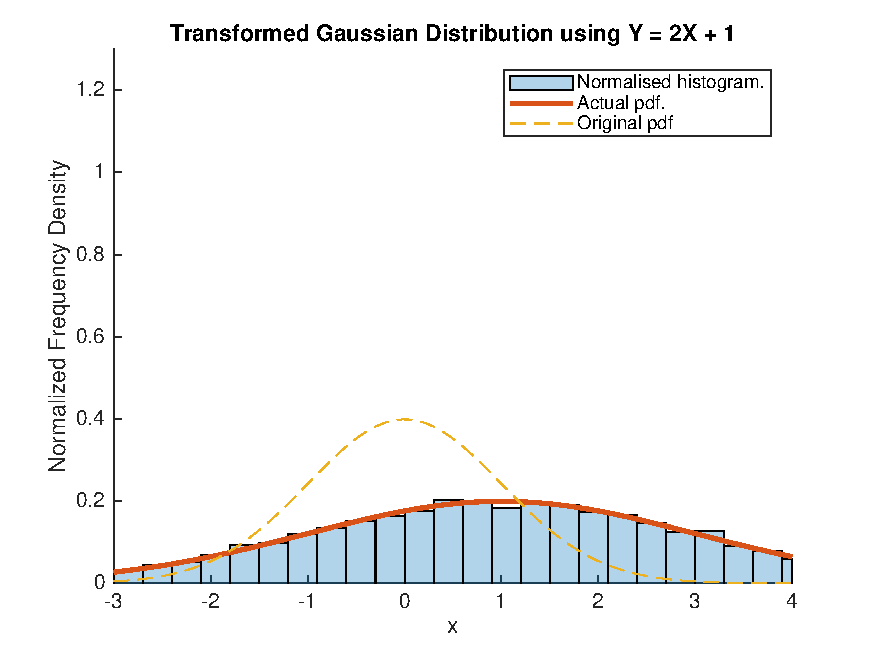
\includegraphics[width=\textwidth]{figures/gaussian-linear-transform.pdf}
  \caption{Histogrammed samples from a ${\cal N}(x|0,1)$ transformed using $f(x) = 2x + 1$ }
  \label{fig:gaussian-linear-transform}
\end{figure}




Now take $p(x)={\cal N}(x|0,1)$ and $f(x)=x^2$. Calculate $p(y)$ using the Jacobian formula:

$f(x) = x^2$. Therefore, $\frac{dy}{dx} = 2x$  and $f^{-1}(y) = \pm \sqrt{y}$. Note $f^{-1}(y)$ is multi valued with ${f_1}^{-1}(y) = \sqrt{y}$ and ${f_2}^{-1}(y) = -\sqrt{y}$.

\begin{align*}
p_Y(y)  &= \left. \frac {p_X(x)} {\left| \frac {dy} {dx} \right|} \right|_{x = {f_1} ^ {-1} (x)}
+ \left. \frac {p_X (x)} {\left| \frac {dy} {dx} \right|} \right|_{x = {f_2} ^ {-1} (x)}
\\ p_Y(y) & = \frac {p_X ( \sqrt y )} {\left| 2 \sqrt y \right|} + \frac {p_X (- \sqrt y)} {\left| - 2 \sqrt y \right|}
\\ p_Y(y) & = \frac {p_X (\sqrt y)} {\sqrt y} = \frac 1 {\sqrt{2 \pi y}} e ^ { - \frac {y} {2}}, y \ge 0
\end{align*}
Where the last line follows because $p_X$ is an even function when $X$ has a Gaussian distribution.


Figure \ref{fig:gaussian-quadractic-transform} shows histogrammed transformed random samples overlaid with the calculated PDF. The strong correlation verifies the above result.


\begin{figure}[H]
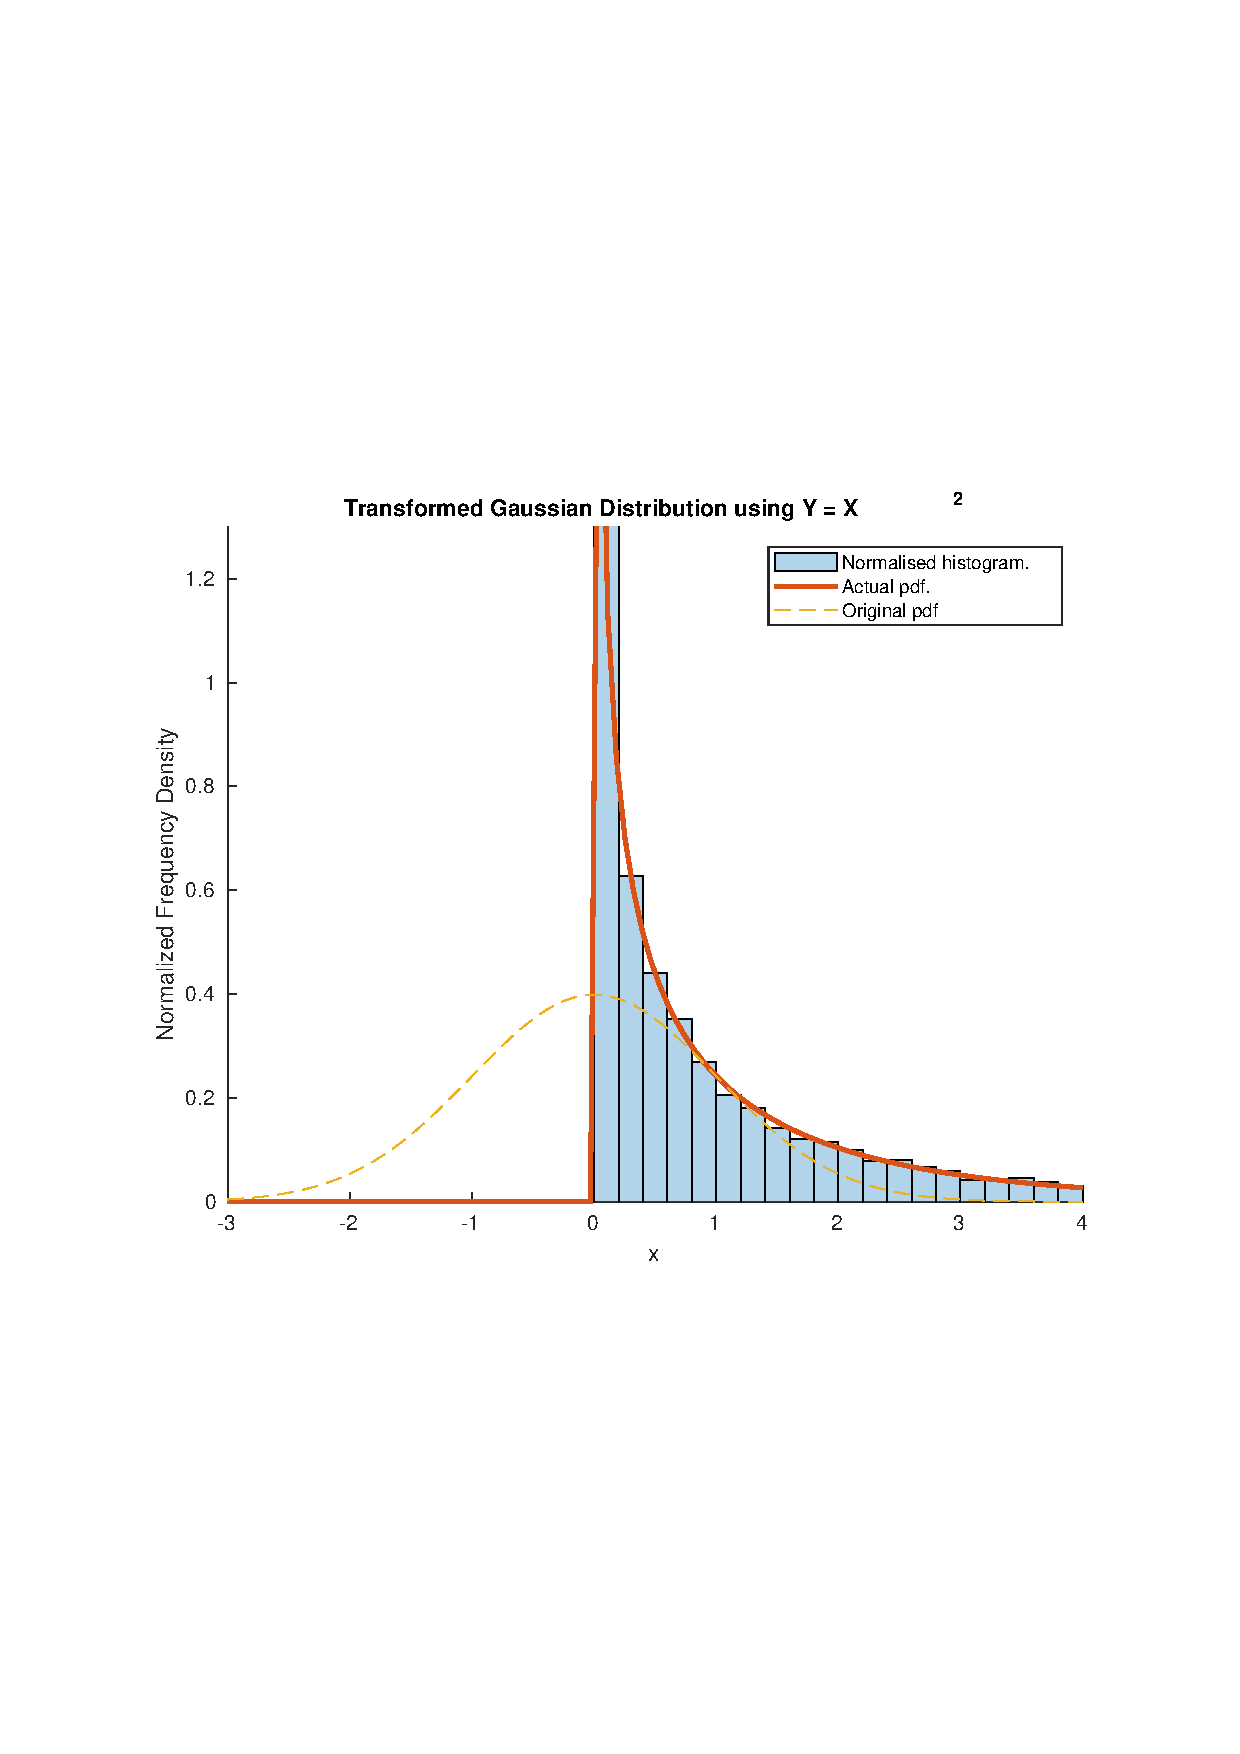
\includegraphics[width=\textwidth]{figures/gaussian-quadratic-transform.pdf}
  \caption{Histogrammed samples from a ${\cal N}(x|0,1)$ transformed using $f(x) = x^2$ }
  \label{fig:gaussian-quadractic-transform}
\end{figure}


\item{\bf Inverse CDF method} 



For an exponential distribution with $\mu = 1$ the PDF $p_Y(y)$ , the CDF $F_Y(y)$ and the inverse CDF ${F_Y}^{-1}(x)
$ are given by:


\begin{align*}
p_Y(y)  &= e ^ {-y}, y \ge 0
\\ F_Y (y) &= \int _ {- \infty} ^ y p_Y (y) \, dy =  \int _ 0 ^ y e ^ {-y} \, dy = 1 - e ^ {-y}
\\ {F_Y} ^ {-1} (x) &= \log {\left( \frac 1 {1 - x} \right)}
\\ y^{(i)} &= {F_Y} ^ {-1} (x ^ {(i)}) = \log \left(\frac 1 {1 - x ^ {(i)}}  \right)
\end{align*}


MATLAB code for inverse CDF method for generating samples from the exponential distribution. Samples generated using this method are shown on the histogram plot in figure \ref{fig:exponential-histogram} and the \code{ksdensity} plot in figure \ref{fig:exponential-ksdensity}.

\begin{lstlisting}[language=MATLAB]
uniform_values = rand(N, 1);
inverse_exponental_cdf = @(x) log(1 ./ (1 - x));
exponential_values = inverse_exponental_cdf(uniform_values);
\end{lstlisting}


\begin{figure}[H]
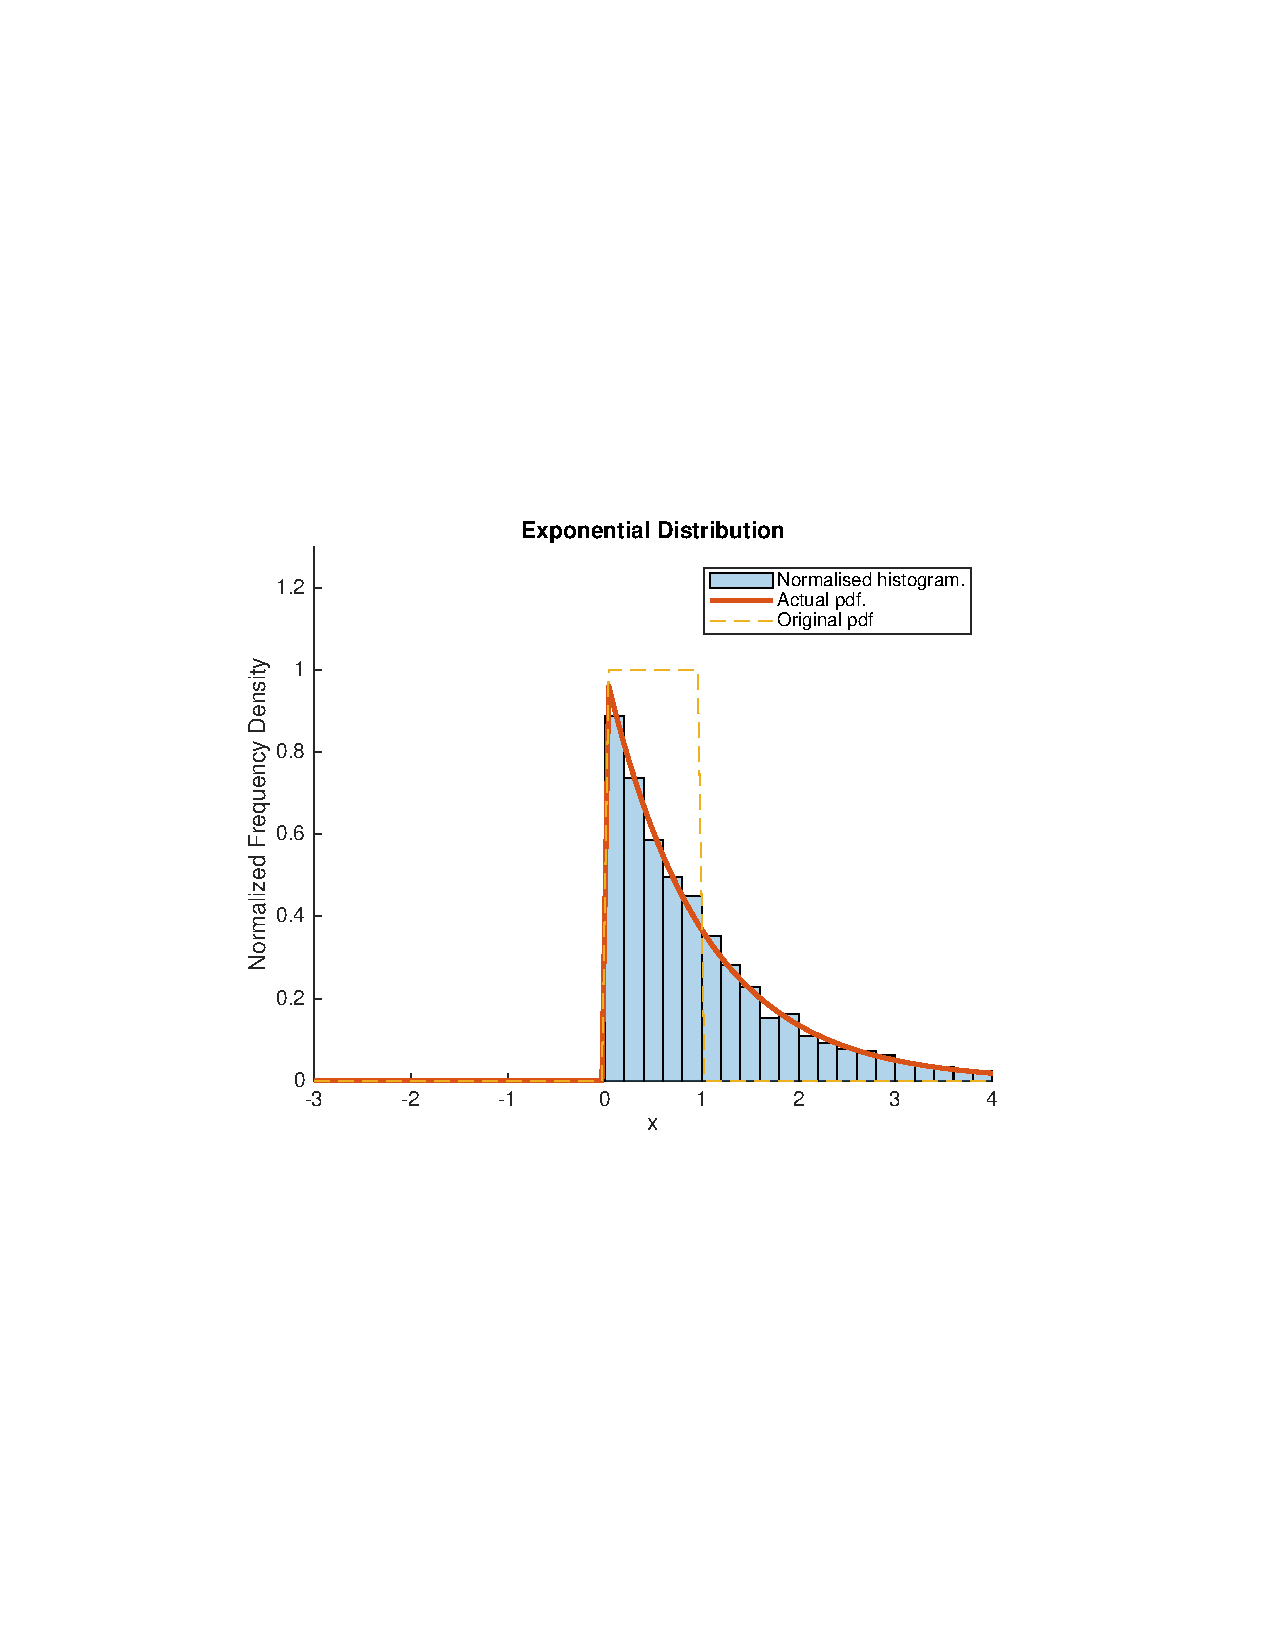
\includegraphics[width=\textwidth]{figures/exponential-histogram.pdf}
  \caption{Histogrammed samples from an exponential distribution generated using the inverse CDF method. }
  \label{fig:exponential-histogram}
\end{figure}

\begin{figure}[H]
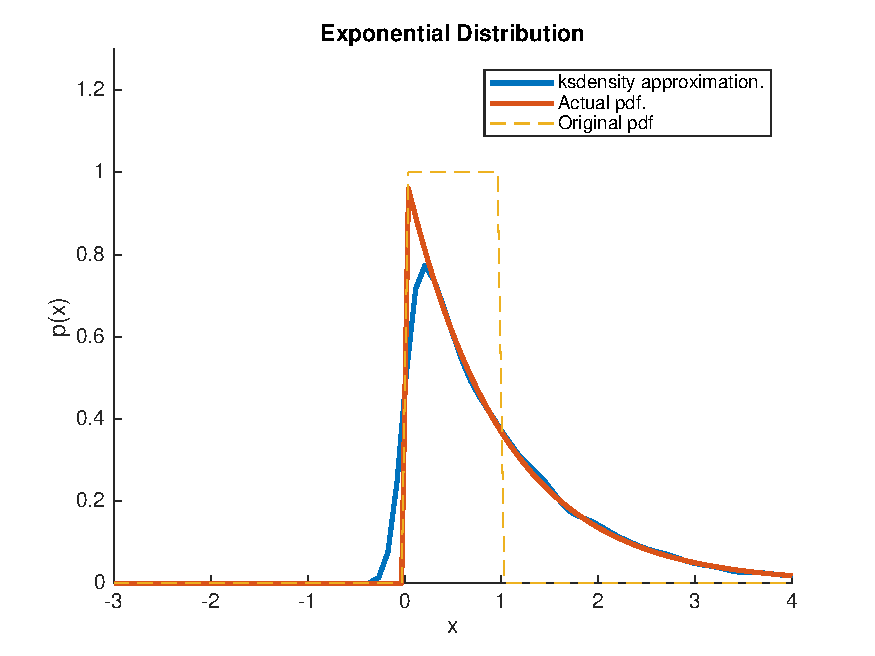
\includegraphics[width=\textwidth]{figures/exponential-ksdensity.pdf}
  \caption{\code{ksdensity} estimate of exponential PDF generated using the inverse CDF method. }
  \label{fig:exponential-ksdensity}
\end{figure}

\item {\bf Simulation from a `difficult'  density.}

For parameters $\alpha$ and $\beta$, the function \code{generate\_alpha\_stable()} converts samples from uniform and exponential distributions into samples taken from the alpha stable distribution.

MATLAB code to generate $N$ random numbers drawn from the distribution of $X$:

\begin{lstlisting}[language=MATLAB]
function X = generate_alpha_stable(alpha, beta, uniform, expo) 
% generate_alpha_stable  Generates an alpha stable distribution.
%   X = generate_alpha_stable(alpha, beta, uniform, expo)
%   alpha and beta are the parameters of the distribution.
%   uniform and expo should be identically sized vectors of uniform and
%       exponentially distributed random numbers which will be used to 
%       generate x.
%   X is a vector of random variables of length equal to the length of 
%       uniform and expo.

    b = 1/alpha * atan(beta * tan(pi * alpha / 2));
    s = (1 + beta^2 * tan(pi * alpha /2)^2)^(1 / (2*alpha));
    
        
    X = s * sin(alpha * (uniform + b)) ./ ...
        cos(uniform).^(1 / alpha) .* ...
        (cos(uniform  - alpha * (uniform + b)) ./ expo).^((1 - alpha) / alpha);
end
\end{lstlisting}

\code{ksdensity} estimates of distribution with $\alpha=0.5,\,1.5$ and several values of $\beta$:

\begin{figure}[H]
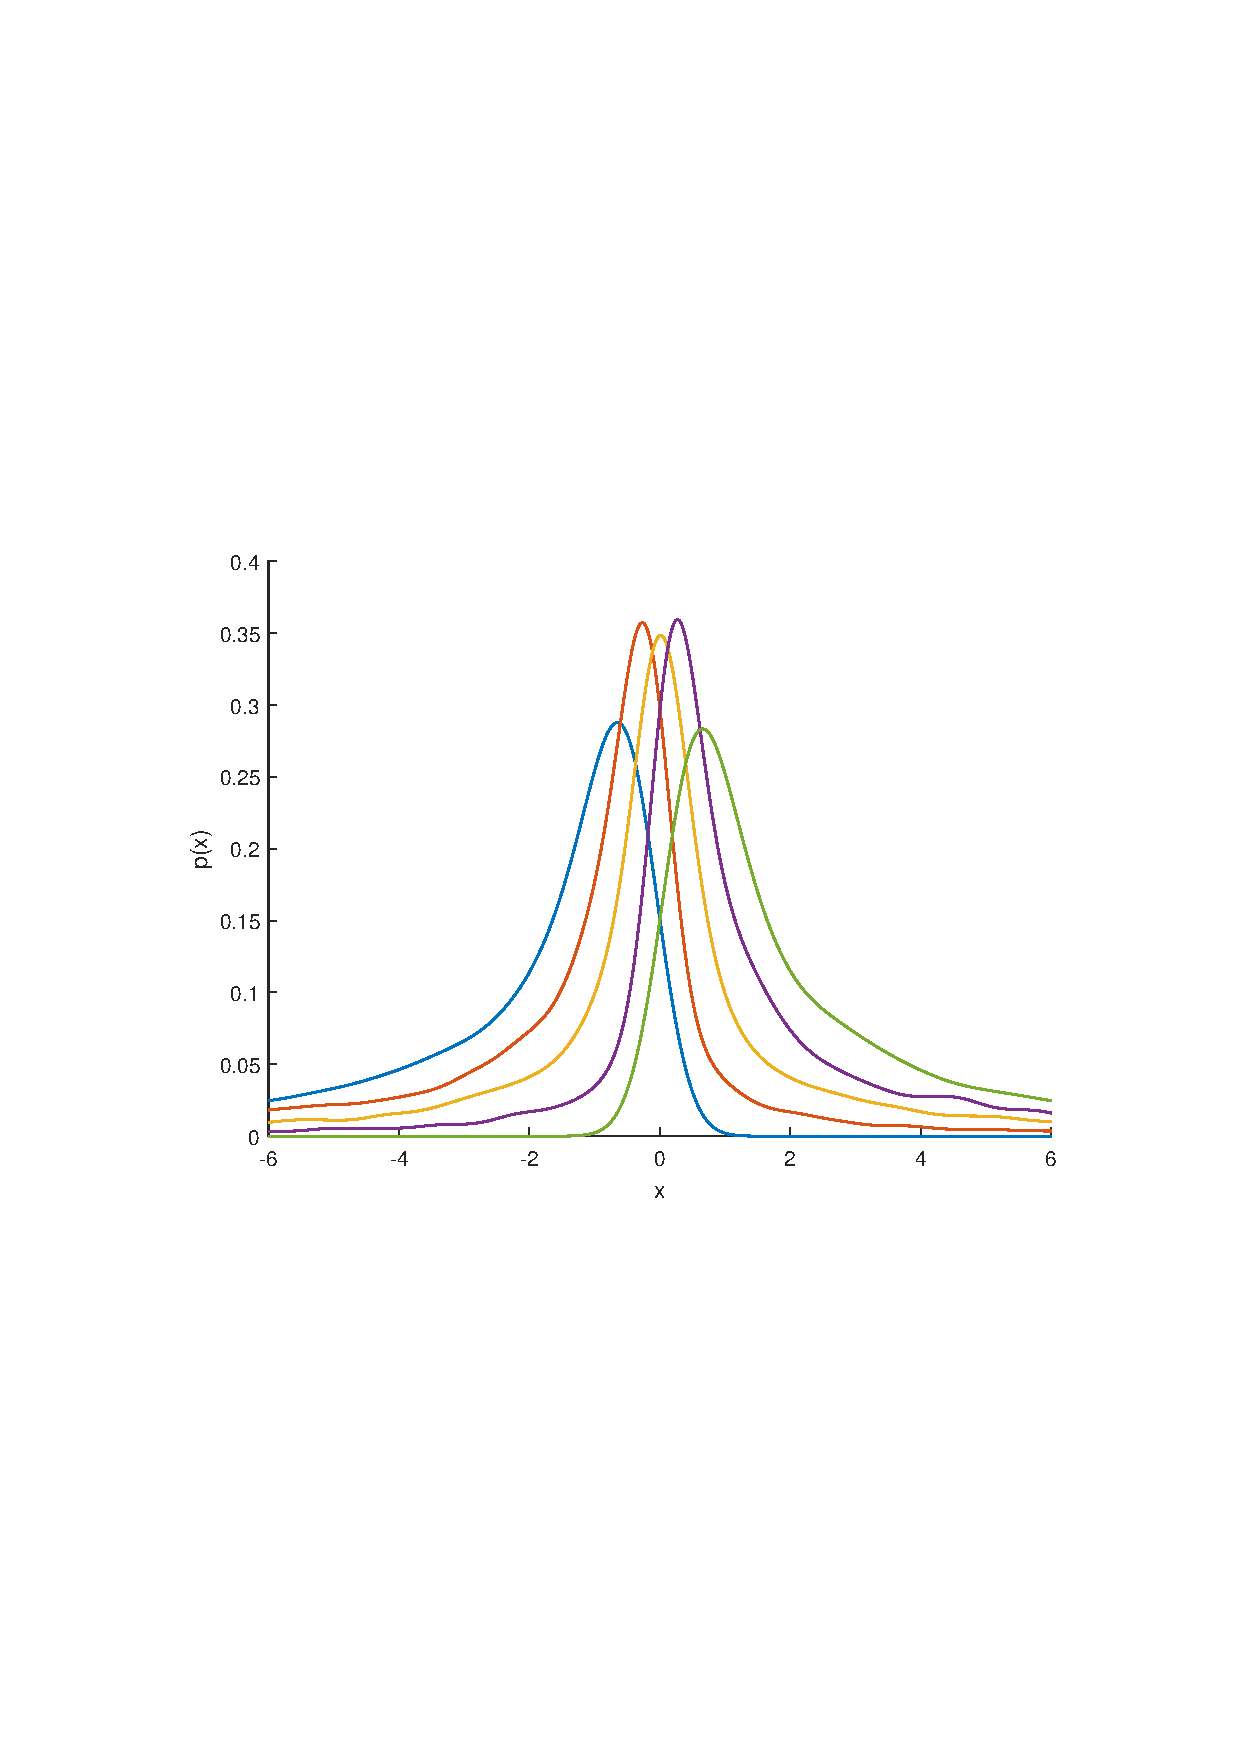
\includegraphics[width=\textwidth]{figures/alpha-0_5-with-several-beta.pdf}
  \caption{\code{ksdensity} estimate of alpha stable PDF with $\alpha = 0.5$ }
\end{figure}

\begin{figure}[H]
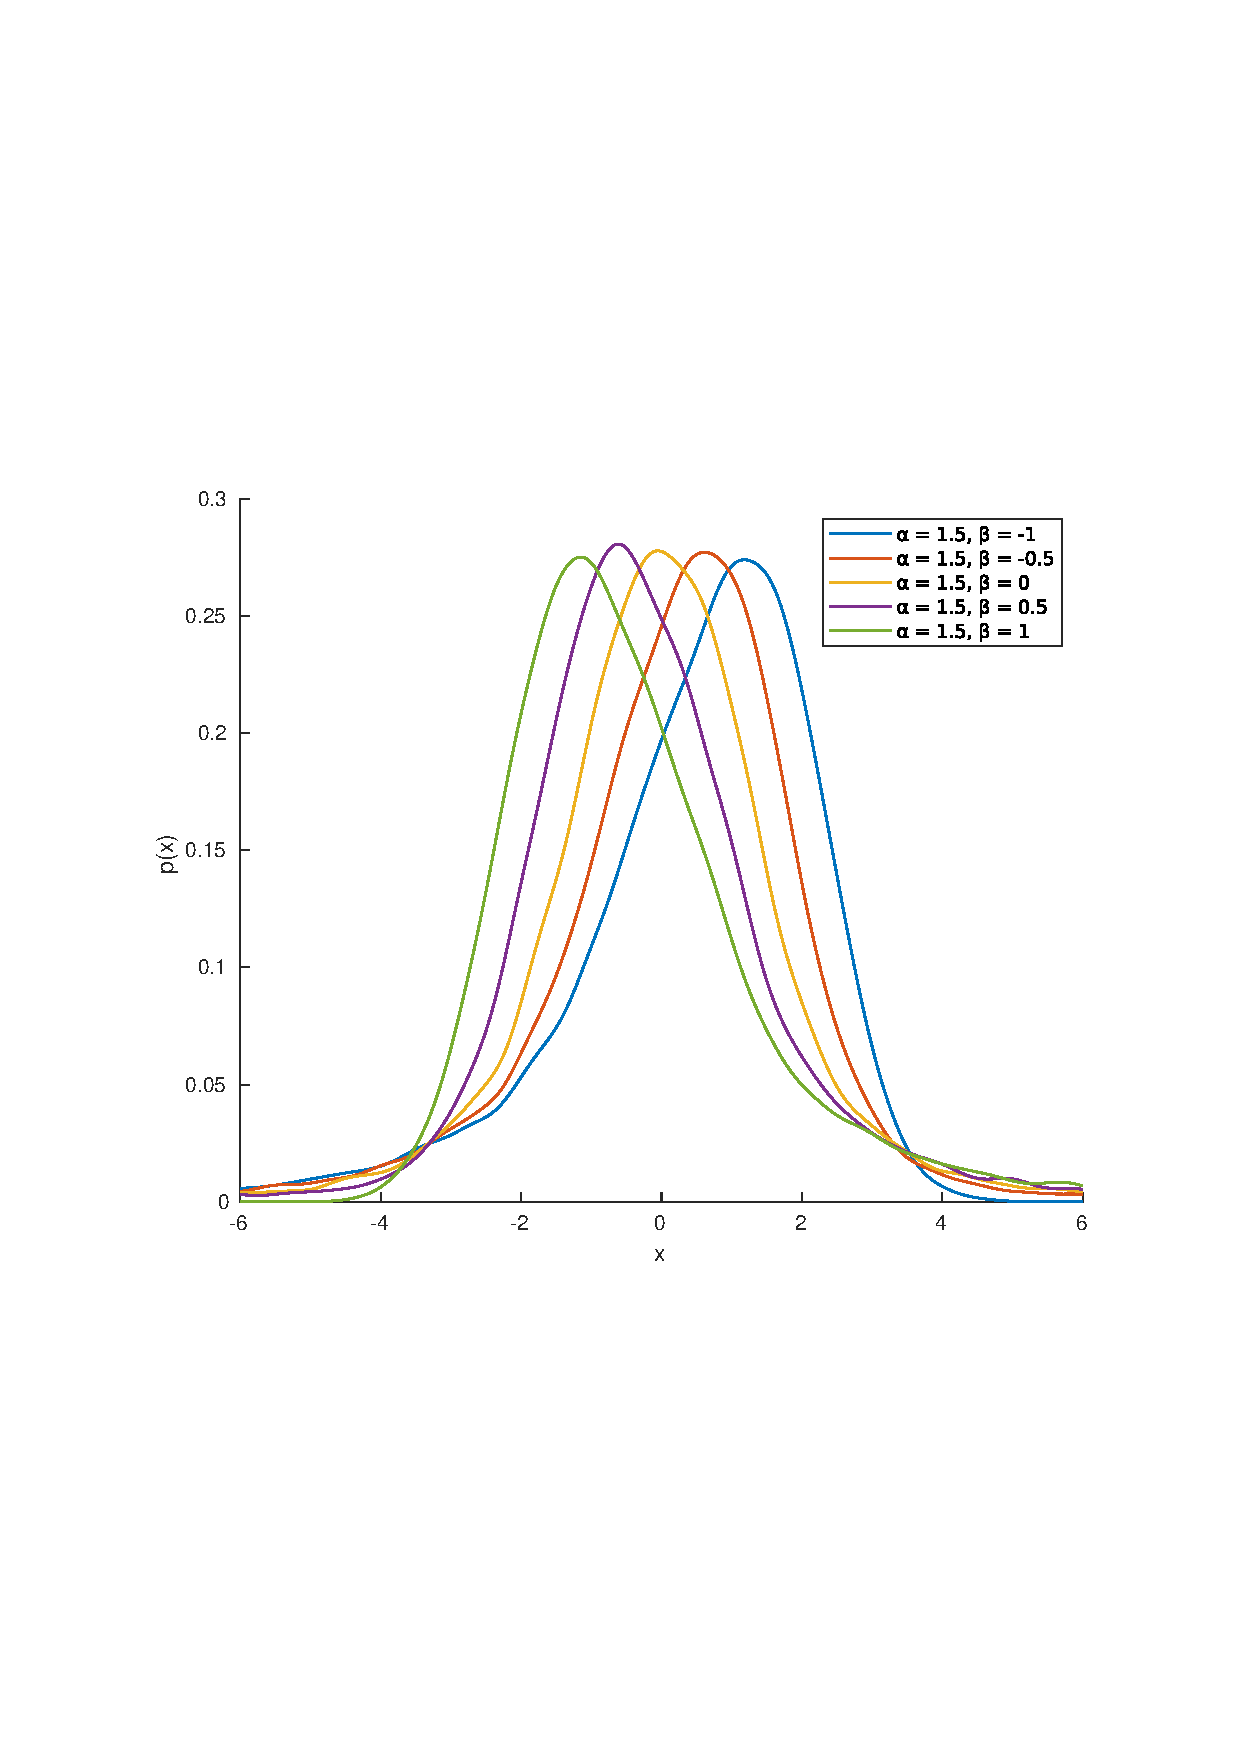
\includegraphics[width=\textwidth]{figures/alpha-1_5-with-several-beta.pdf}
  \caption{\code{ksdensity} estimate of alpha stable PDF with $\alpha = 1.5$ }
\end{figure}

\code{ksdensity} estimates of distribution with $\beta=0,\,1.5$ and several values of $\alpha$:

\begin{figure}[H]
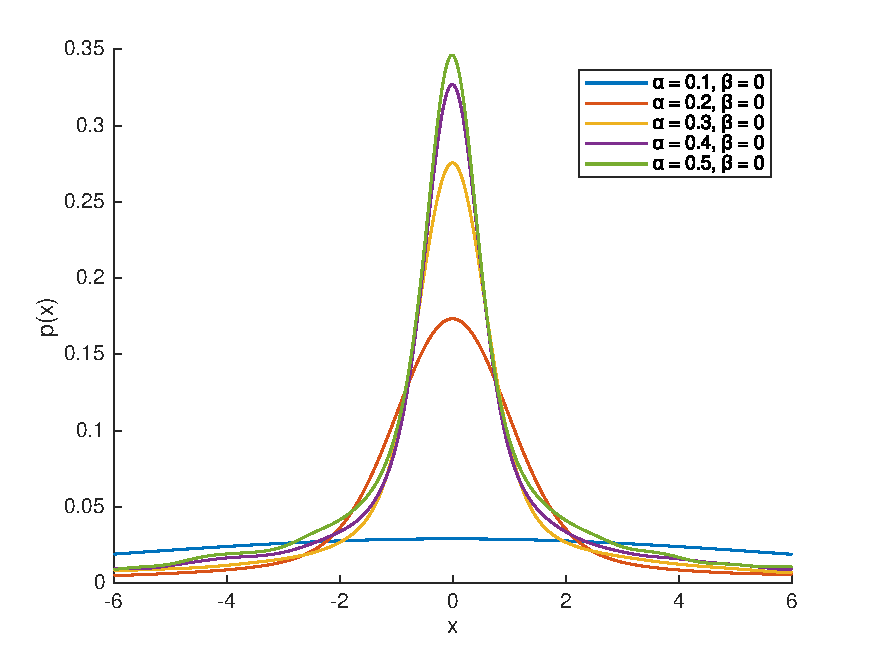
\includegraphics[width=\textwidth]{figures/beta-0-with-several-large-alpha.pdf}
  \caption{\code{ksdensity} estimate of alpha stable PDF with $\beta = 0$ and $\alpha \ge 0.5$ }
\end{figure}

\begin{figure}[H]
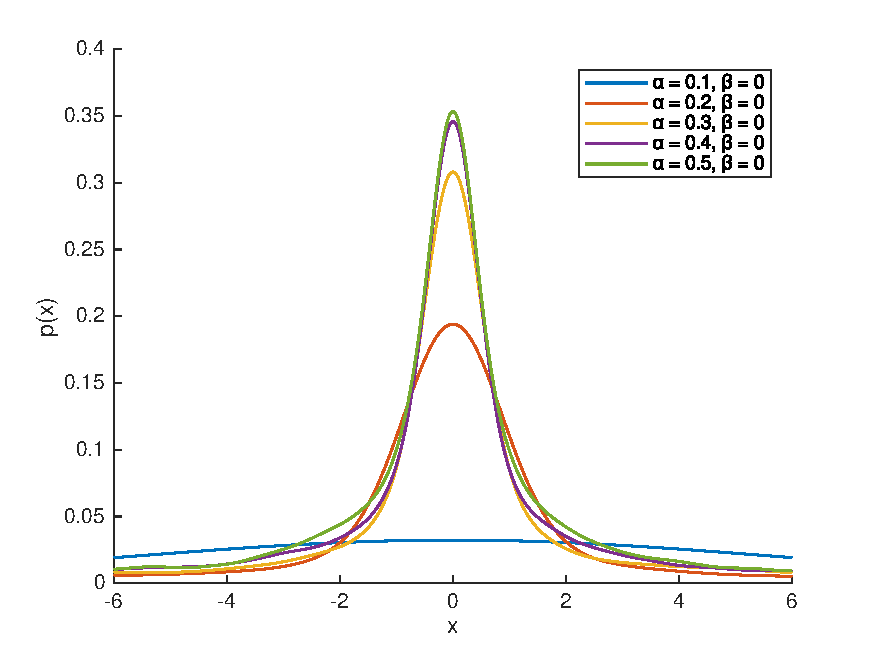
\includegraphics[width=\textwidth]{figures/beta-0-with-several-small-alpha.pdf}
  \caption{\code{ksdensity} estimate of alpha stable PDF with $\beta = 0$ and $\alpha \leq 0.5$ }
\end{figure}

Parameters $\alpha$ and $\beta$ define the shape of the distribution. $\beta \ne 0$ causes the distribution to be skewed. $\beta > 0$ causes the distribution to be very steep for the left side and then very shallow on the right side, as $\beta \to 1$ the distribution becomes very heavy tailed. The opposite (heavy tail on the left side and sharp cut off on right side) is true for 

$\alpha$ controls the variance of the distribution, $\alpha=1/2$ creates a very sharp distribution which broadens out as $\alpha$ decreases or increases. In the limit as  $\alpha \to 0$ the distribution becomes  0 everywhere (whilst integrating to unity).

\end{enumerate}



\end{document}



\end{document}


